\documentclass{article}
\usepackage[utf8]{inputenc}
\usepackage{graphicx}
\usepackage{minted}
\usepackage{hyperref}
\usepackage[T1]{fontenc}
\title{Comparing collections of Rijksmusuem and Moma using knowledge grpahs}



\author{
  Pawel Piwowarski\\
  \texttt{2729221@student.vu.net}
  \and
  Adam Rydzinski\\
  \texttt{2739038@student.vu.nl}
  \and
  Keira Zieboll\\
  \texttt{}
   \and
  Teodora Taran\\
  \texttt{2737833@student.vu.nl}
}


\date{Group\_99 on October 28 2022}

\begin{document}

\maketitle


\section{Introduction}
\subsection{Defining the goal of our analysis}

Our analysis is primarily focused on works of art curated by the Museum of Modern Art (MoMA) in New York and the Rijksmuseum in Amsterdam. It aims to collect and display information in a visual manner, with regards the works of art contained within these museums. We would like to show the differences and similarities between the artworks of the two museums in categories such as, artists characteristics and the time period in which the artworks were created. We’d like to visualize these in order to make it easier to compare how the two museums differ, and to show what aspects of the artworks are most and least prevalent among the datasets we have gathered.


\subsection{Identification of the Stakeholders}

Given that our analysis aims to provide a comprehensive overview of the different types of artworks located in the MoMA and the Rijksmuseum, the main stakeholders are tourists and other travel providers. Tourists can use the information provided by the analysis and visualization in order to better inform their travel plans, by showing them the museum location they should visit in order to find artworks corresponding to their preferred genre or period. Furthermore, travel providers such as travel agents and tour companies can use this information to construct personalized tour packages for their customers, which will increase firm revenue through improvements in customer value proposition \cite{keira}.

A secondary consequence of this analysis is that determining the most suitable museum to visit may also reduce the negative environmental effects of tourism. By recommending only the museum that fits the tourist’s interests, the tourist will be less likely to want to visit other museums that they will not be as satisfied by, thereby reducing carbon emissions from (air) transportation to the museum location.

\subsection{Designing the Analysis}

The analysis is a comparison of artworks and artists from both museums and which sort of periods and nationalities are the most prevalent in a given museum. We want to analyze the data by means of visualization using the pandas and folium libraries in python.  The first step of our analysis would be to specify the factors that we want to compare between both museums. We then create visualizations showcasing these differences. Lastly, we draw conclusions from the visualizations and summarize our work. The visualizations that we want to provide will focus on displaying information such as the period of a particular work of art or the birth date of the artist as well their nationality. We also want to create an interactive way of displaying the artworks based an a particular year or a name of the artist.

For the statistical information regarding nationalities and the data concerning the periods of artists we want to utilise bar-graphs or pie graphs which will help visualise which museum has the biggest impact on a given value f.e which museum has the most works from the year 1882.

As for the interactive visual information about the artwork we want to create a simple search mechanism were users can present their search criteria and based on them an artwork will be displayed.

\subsection{Motivation of Ontology Choice}


We chose our ontologies based on how suitable they were for use with our domain of choice. We wanted to describe specific aspects of artworks, the artist responsible for the creation of the artwork and the location where it is currently kept. Our first ontology was the GeoSPARQL ontology\cite{GeoSparql} which was able to support geolocation data for each of our artworks it will be also useful for categorizing artworks as spacial objects and nationalities as abstract concepts. We also used the FOAF\cite{Foaf} vocabulary through which we were able to create artists as persons. Lastly we used the dbo:Artwork ontology\cite{Artwork} for creating the sub-ontology for our all of our artworks.


\subsection{Description of External Datasets}

Similarly to our choice of ontologies, we found appropriate datasets that would fit our analysis domain. We narrowed down our choice of external datasets to 3 different sources: the MoMA data service\cite{Moma}, the Rijkmuseum data service\cite{Rijks} and DBPedia, which is the external SPARQL endpoint\cite{Dbpedia}. 

With an ever-changing collection of around 200,000 pieces from all over the world, painting, sculpture, printing, drawing, photography, architecture, design, video, media, and performance art are among the many forms of visual expression represented in the collection of MoMA.
Each work has associated basic metadata, such as its title, artist, date of creation, medium, size, and the date of acquisition by the Museum." The artists dataset comprises 15,091 entries, which reflect all of the artists whose work is in the MoMA collection and has been cataloged in the database. Each artist's basic metadata is included, such as their name, country of origin, gender, birth year, and death year.

Likewise, the data services of the Rijksmuseum enable access to object metadata, bibliographic data, controlled vocabularies, and user contributed material. The data which is found in this dataset, similar to the one of MoMA, displays ranging types of information about artworks such as their title, artist, date of creation and category of art.

Lastly, DBpedia qualifies for querying relationships and properties of Wikipedia resources, including links to other related datasets.


\section{Domain Modeling and Data Integration}


\subsection{Domain and Scope of the Ontology}


The data domain of our project is mainly focused on artists and artworks displayed at the
Museum of Modern Art (MoMA) in New York and the Rijksmuseum in Amsterdam. What we
hope to deliver is an understanding of how information regarding the artworks exhibited in both
museums compare to one another by providing a visual representation of the data in our domain.
Through ontology alignment, we determined correspondences between concepts in two
previously found ontologies. The Dbpedia Artwork has information relevant to the vocabulary
of artworks, which with the addition of some supplementary class including FOAF:person , manages to link them
to the artists responsible for their creation. The GeoSPARQL ontology is able to concepts related to the tangiblity of the objects.

\subsection{Methodology Description}


When it comes to the methodology concerning our ontology, our main rule was to create an
ontology that is as intuitive as possible, we also wanted to allow for a rich use of the imported
ontologies through mapping constructs. Additionally we wanted to infer rich information that will prove
to be crucial in the domain of our ontology. We knew from the beginning that our ontology will
use a more substantial amount of properties than classes, since our data does not differ greatly by
type but rather by the properties it has. The main factor that played a big role in the
creation of the ontology was the correct alignment of the classes and properties with the datasets
provided by external sources.

\subsection{Domain Conceptualization}
For clarity of the presentation each class will be \underline{underlined} and each property will be writen using \textit{italics}. 
In our model, we have defined two main classes,  \underline{Artist} and \underline{Artwork}. These classes encapsulate the most important concepts in our ontology. They are subclasses of \underline{Person} and \underline{Spatial Object} respectively. 
Another important class is the \underline{Museum} class which will have two instances "RijksMuseum" and "Moma". Another important classes are the \underline{Country} and \underline{City} classes.  There exists an Object property \textit{lies\_in} which has as the domain \underline{City} and as the range \underline{Country}. Another object property is  \textit{born\_in} which has as the domain class \underline{Person} and has range \underline{City}. Furthermore there exists data properties  \textit{bornat}     and \textit{hasName} with both having \underline{Person} as the domain and respectively xsd:nonNegativeInteger and rdfs:Literal as ranges.
\underline{People} also \textit{hasGender} which is a rdfs:Literal. As for the artists data properties they have \textit{hasOccupation} property. The \underline{Artwork} class has these data properties \textit{hasDimensions}, \textit{hasDimensions}, \textit{hasUrl}, \textit{hasTitle}, \textit{hasMaterials}, \textit{hasColors} with all of these data properties having rdfs:Literal as range. A very important object property is the \textit{made} property which has as domain \underline{Artist} and as range \underline{Artwork}. 

\begin{center}
\subsubsection{Classes}
\newline
\newline
\includegraphics[width=130]{figure_1.png}
\newline
\caption{Figure 1: Class relation hierarchical graph.}
\end{center}


\begin{center}
\subsubsection{Data properties}
\newline
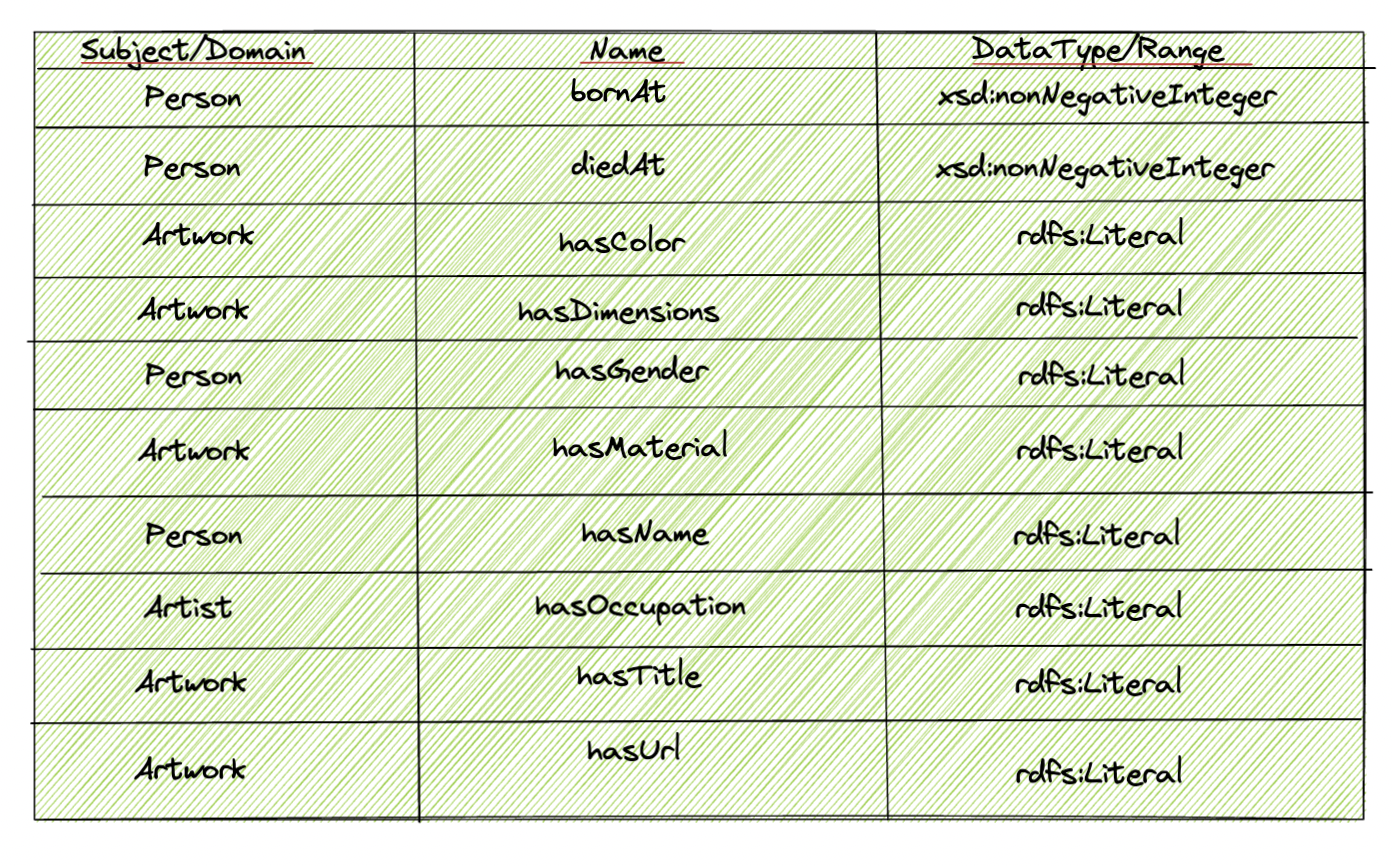
\includegraphics[width=350]{dataproperties.png}
\newline
\caption{Figure 2: Table of data properties in our ontology.}

\newline
\subsubsection{Object properties}
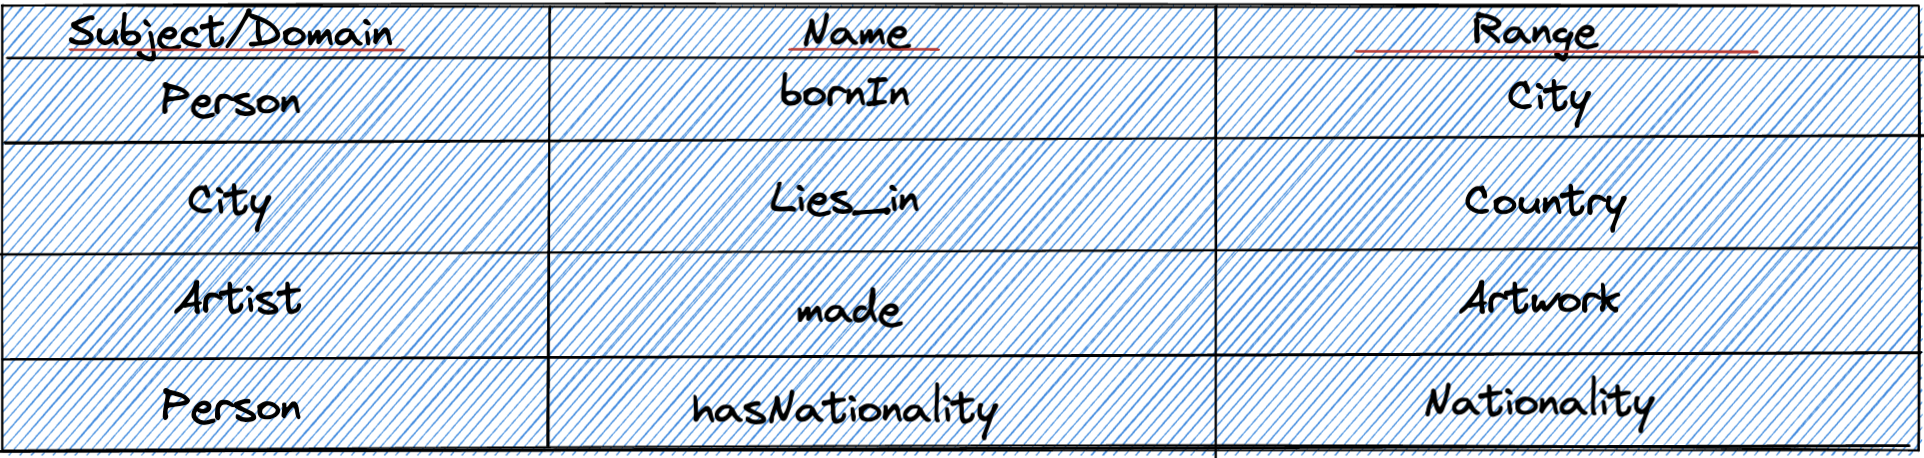
\includegraphics[width=350]{objectproperties.png}
\newline
\caption{Figure 3: Table of object properties in our ontology.}

\newline
\subsubsection{Relation Graph}
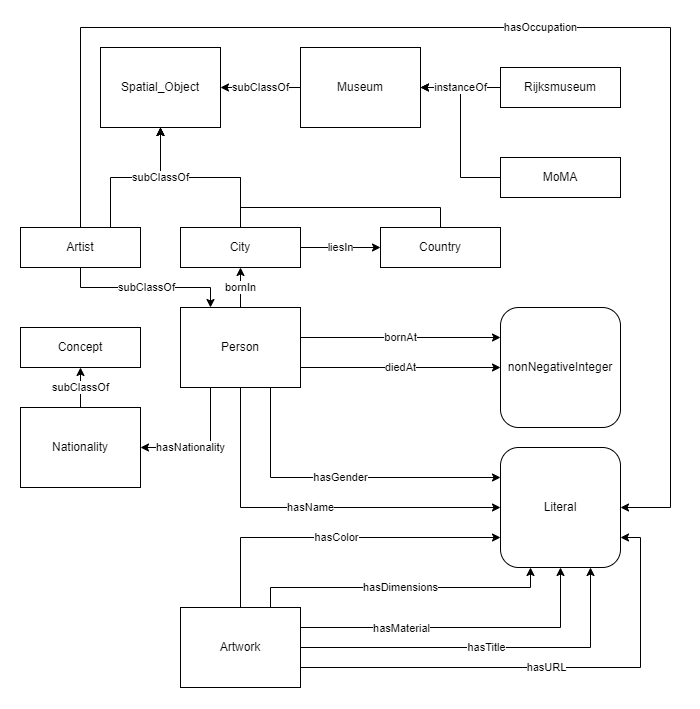
\includegraphics[width=350]{Relation_Graph.png}
\newline
\caption{Figure 4: Relation Graph of every class, data and object property.}
\end{center}


\newpage
\subsection{Ontology Reuse}
Our ontology makes use of 3 existing ontologies. GeoSPARQL ontology for capturing the
geographical presence of our objects. A second ontology dbo:Artwork, from which we reused
the wording of concepts. The third ontology is FOAF for description of personhood of artists.

By reusing the ontologies we’ve created, we added \underline{dbo:work} as a subclass of \underline{geo:SpatialObject}, we
also added a class Museum as a subclass of \underline{geo:SpatialObject} as well as Country and City classes.
Another subclass relationship is that of the Artist class being a subClassof \underline{Person} class, which is
equivalent to the \underline{Foaf:Person} class. There also exist two subclasses of the concept taken from the
GeoSPARQL vocabulary, Gender and Nationality. We also added an equivalenceClass relation between the class \underline{Artwork} and \underline{dbo:Artwork}
We also created mapping constructs
using the subClassOf relationship with the GeoSPARQL ontology, mainly \underline{Museum}, \underline{Artwork},
Country and City, which are all subclasses of the \underline{geo:SpatialObject} metaclass mapped from
GeoSPARQL. 

\subsection{Class Restrictions Overview} 
The final step before populating our ontology with relevant data was to create class restriction from which we could draw meaningful inferences. 
\newline
\newline
The first restriction that we thought would be beneficial for our ontology is the necessary and sufficient restriction on the class \underline{Artist}. Mainly that the \underline{Artist} \textit{made} some
\underline{Artwork}
\begin{center}
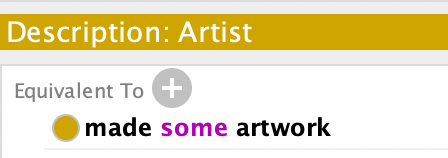
\includegraphics[scale=0.5]{first_restriction.png}
\end{center}
\newline
\newline
The second restriction that we made in our ontology is the necessary and sufficient restriction on the class
\underline{Person}. Mainly that the \underline{Person} \textit{bornAt} some
\underline{xsd:nonNegativeInteger}
\begin{center}
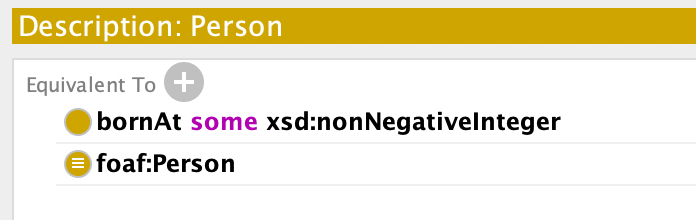
\includegraphics[scale=0.35]{second_restriction.png}
\end{center}
\newline
\newline
The final restriction that we made in our ontology is the necessary and sufficient restriction on the class
\underline{City}. Mainly that the \underline{City} \textit{Lies\_in} some
\underline{Country}
\begin{center}
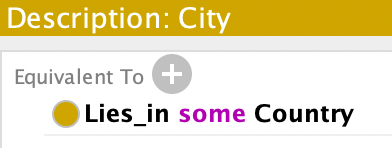
\includegraphics[scale=0.5]{third_restriction.png}
\end{center}




As a result of all of the previous steps, a base ontology
called base.ttl was created, this ontology will become populated with data from both of our
sourced Datesets.
\subsection{Integration of External Datasets and Populating our Ontology}
Since the data that was made available for us was not entirely homogeneous in characteristics we needed to prepossess the data and make the csv files that combined different data sources,

\subsubsection{Rijksmuseum - Artist Ontology}
The main .csv file which we decided to integrate with our ontology is located on the
Rijksmuseum Github \cite{Third_Github}
. The data proved to contain a lot of unnecessary fields. Therefore, we
decided to extract only the most relevant information. The extraction script can be accessed on our
Github \cite{First_Github}
. We used both the SPARQL DBPedia endpoint alongside the standard REST API
provided by the Rijksmusuem \cite{Rijks_Api}with an API key 
. The final .csv files which were used as a base
for the ontology of artists whose works are exhibited at Rijksmusem is found once again in our
Github \cite{Second_Github}
. To build an ontology based on this data, we used a simple python script which opens
the base ontology base.ttl and populates it with the data from the .csv file \cite{lolGith}.

\subsubsection{ Rijksmuseum - Artwork Ontology}
The Artwork ontology for Rijksmuseum was created in a similar manner to the artist ontology. First a script to
extract all of the relevant data to the .csv file was written \cite{Fourth_Github}. Based
on this, the ontology that combines both artists and artworks from Rijksmuseum was created\cite{lolGith2}. 

\subsubsection{ MoMA - Artist Ontology}
We used a similar approach to create the MoMA artist  \cite{Fith_Github}. This time we also used a
SPARQL endpoint at the level of the creation of the knowledge graph itself. Since we wanted to
convey all of the information necessary for a homogeneous dataset, we queried information
regarding the birthplaces of specific artists based on their name and occupation. The code
requires around 15,000 artists to process it through the endpoint. It takes around 30 minutes for
the final knowledge graph with MoMA artists to be outputted.

\subsubsection{Moma - Artwork Ontology}

The creation of Artwork ontology for Moma was the easiest piece of the puzzle, it just required to write a simple python script which used the .csv file which proved to suit our needs \cite{Sixth_Github}. 

\newpage
\subsection{Inference Description}

The first inference that the reasoner picked up correctly inferred that all entities with the bornAt
predicate are Persons. When we created the class restriction that every entity that was bornAt
some date is a Person, the reasoner correctly inferred that all of the entities that we added to the
graph are in fact Persons.The second inference was that Artist is an equivalence class of Person. This is simply because
there are no other entities with the bornAt relation in our ontology 

\begin{center}
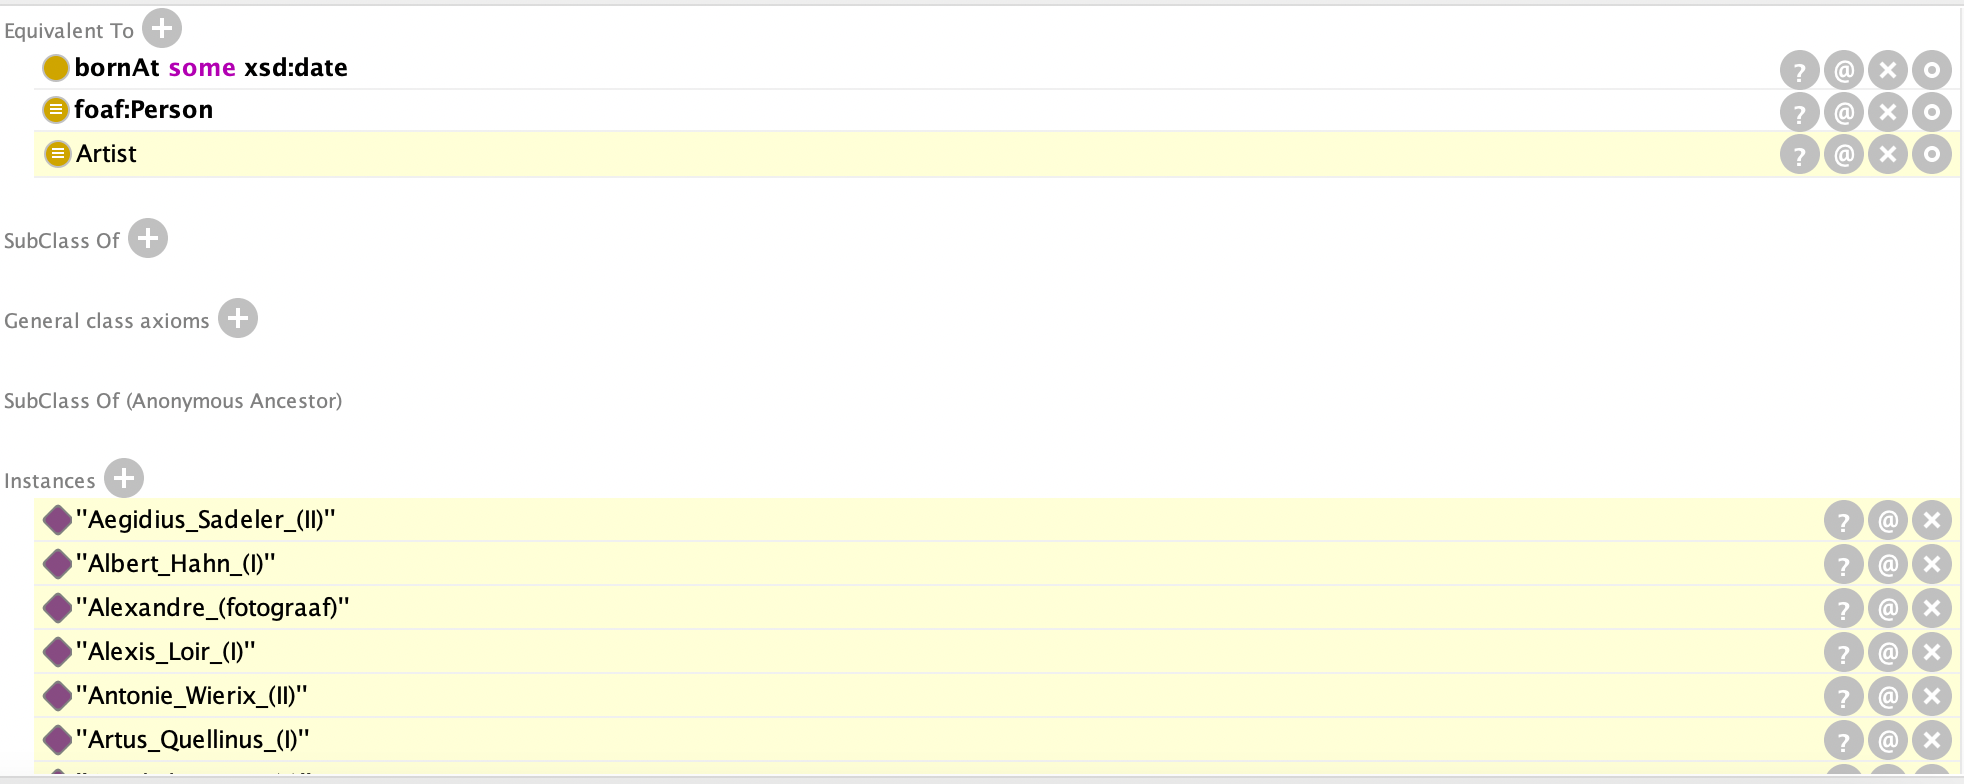
\includegraphics[width=350]{first_inference.png}
\newline
\caption{Figure 5: Reasoner inferring that all entities with "bornAt" predicate are "Persons".}
\end{center}


\newpage
The third inference that we noted was that every entity that made an artwork is an artist. This
is definitely the case.
\begin{center}
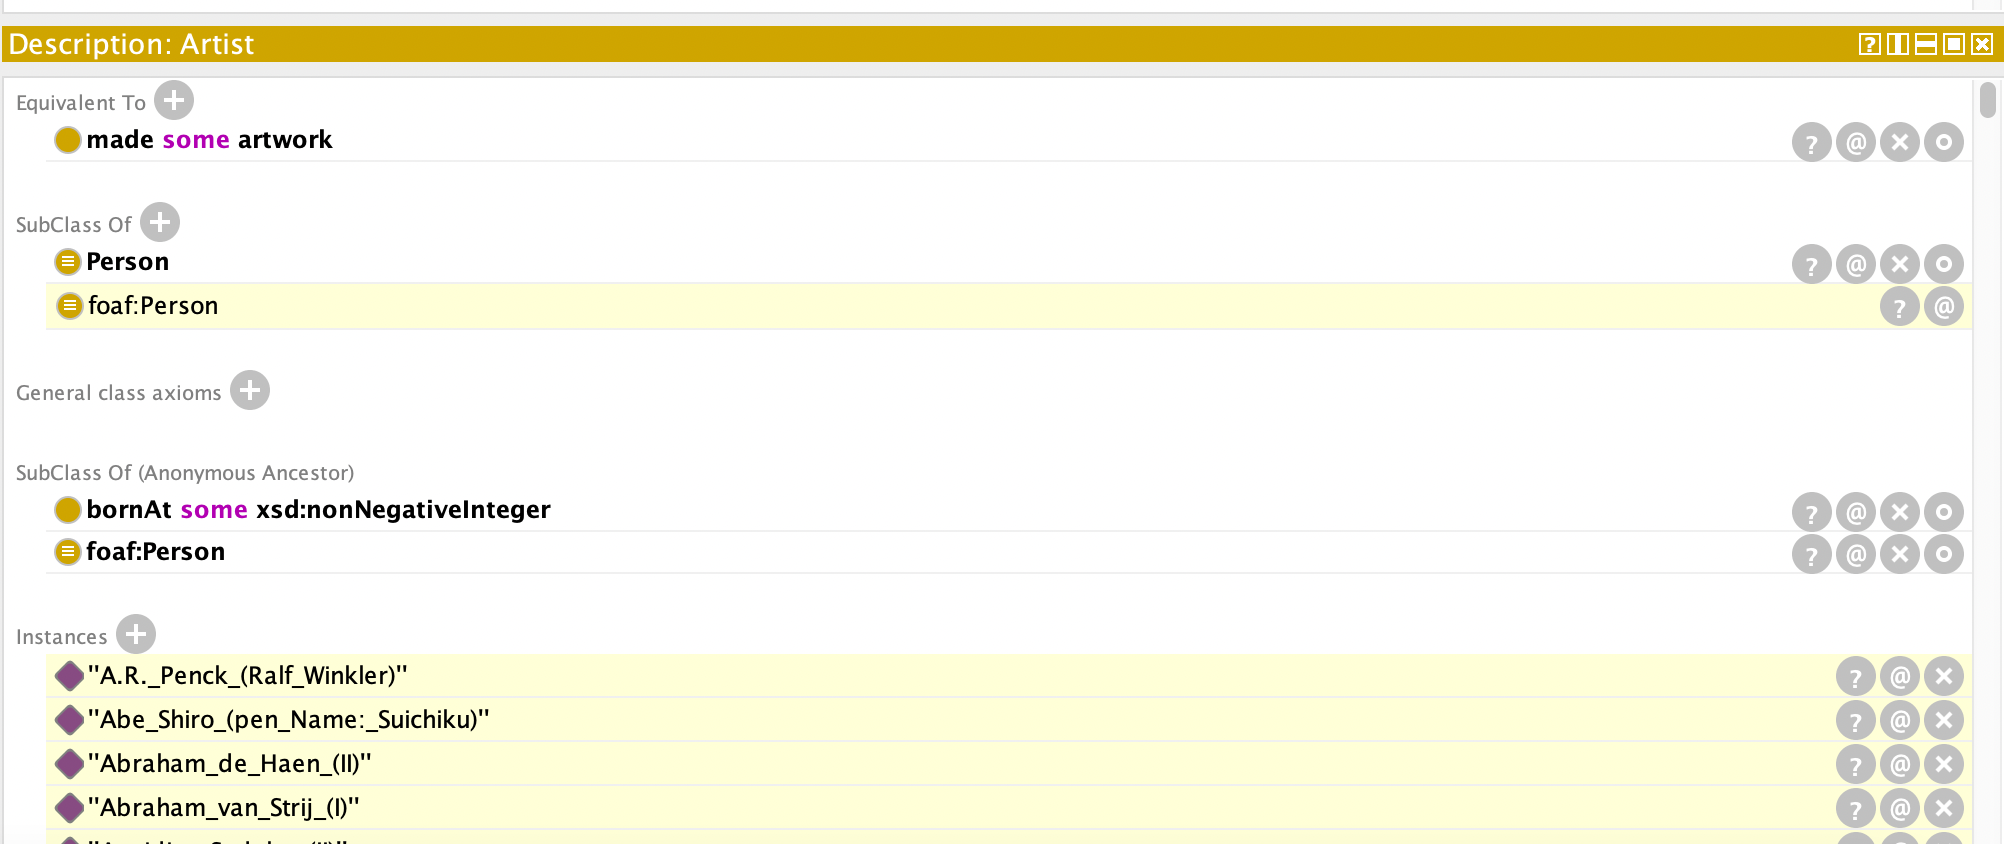
\includegraphics[width=350]{second_inferece.png}
\newline
\caption{Figure 6: Reasoner inferring that all entities which "made some artwork" are artists.}
\end{center}

The fourth inference that we noted was the inference based on the domain and range restrictions. The class \underline{Nationality} is populated with instances because of the restriction that \textit{hasNationality} has the range \underline{Nationality}
\begin{center}
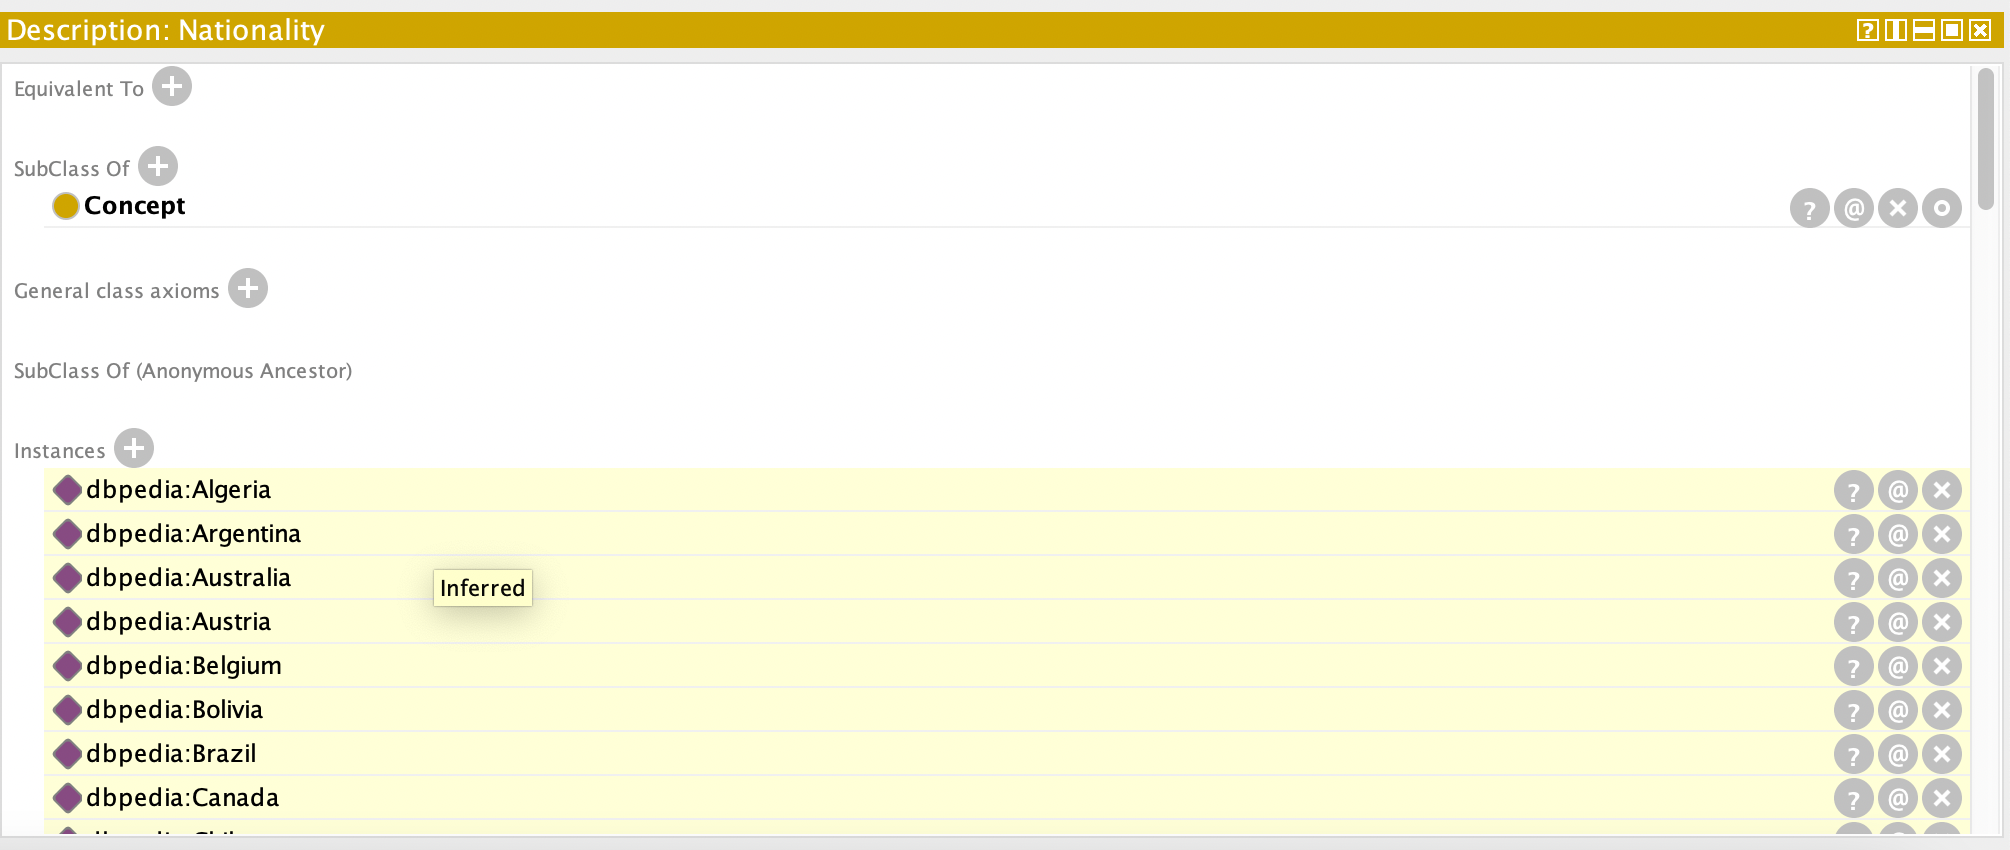
\includegraphics[width=350]{fourth_inference.png}
\newline
\caption{Figure 7: Class "Nationality" is populated with instances.}
\end{center}
\newline
The last inference that we wanted to include is the inference on the class \underline{City}, mainly all of the entities that that have the \textit{liesIn} relation have to be a city (based on the domain/range characteristics).

\begin{center}
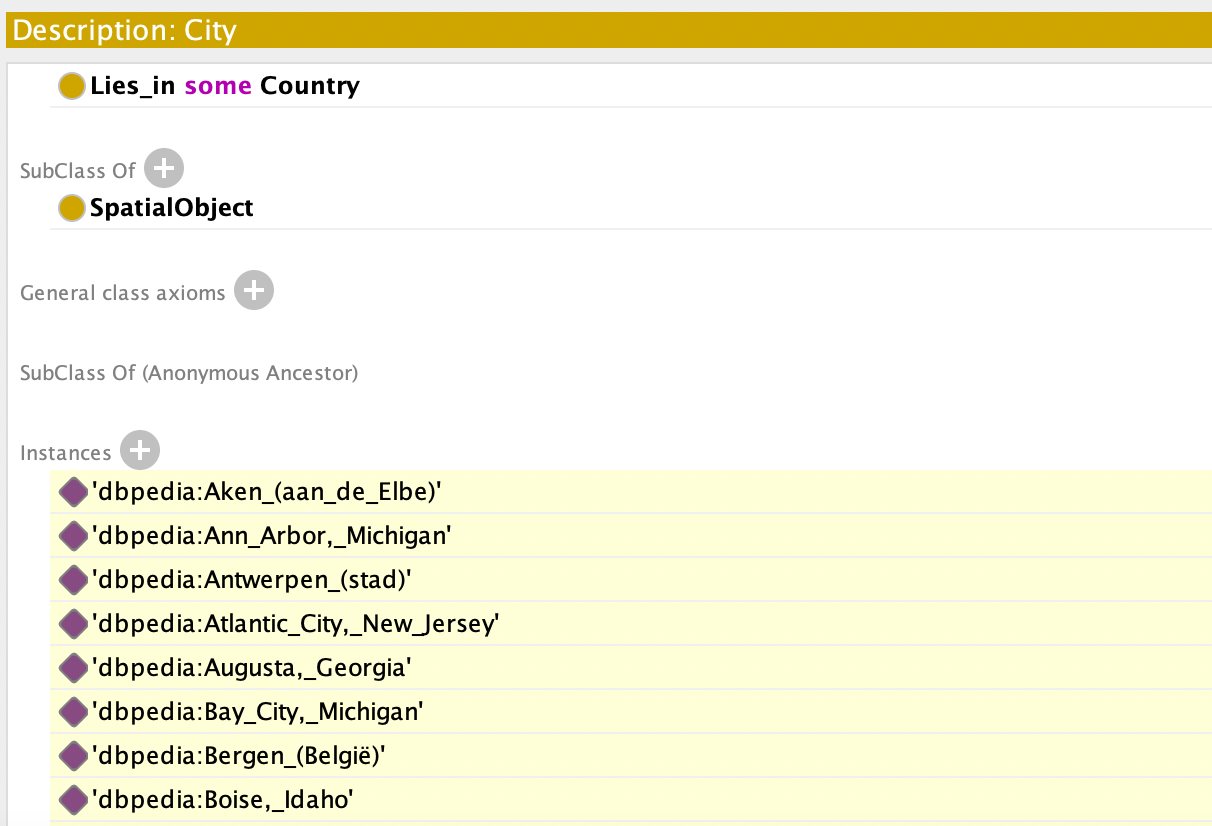
\includegraphics[width=350]{third_inferece.png}
\newline
\caption{Figure 8: All entities with "liesIn" relation are in class "City".}
\end{center}
This inferences are very crucial for our final ontology, that is why we have exported them and added them to
the final .ttl file which we have added to GraphDB. And this file will be the ontology against which we'll execute our SPARQL queries.

\subsection{SPARQL Queries}

We made a lot of choices concerning the final shape of the characteristics that we wanted to extract from our dataset. All of the queries reflect our initial intention. 

\subsubsection{Counting all Artworks}
The first query that we judged to be relevant is getting the number of works located at both museums. 
\begin{minted}{sparql}

PREFIX art: <http://www.semanticweb.org/ontologies/2022/9/group_99#> 
PREFIX owl: <http://www.w3.org/2002/07/owl#> 
PREFIX rdf: <http://www.w3.org/1999/02/22-rdf-syntax-ns#> 
PREFIX xml: <http://www.w3.org/XML/1998/namespace> 
PREFIX xsd: <http://www.w3.org/2001/XMLSchema#> 
PREFIX rdfs: <http://www.w3.org/2000/01/rdf-schema#> 


SELECT  ?museum  (count(?x) as  ?number_of_artworks) WHERE { 
?x art:locatedIn ?museum .
}

GROUP BY(?museum)
\end{minted}


\subsubsection{Nationality Data for Artists}

The other interesting query that we needed was the query for getting the nationality of each artists that made works that are locatedIn each of the museums.

\begin{minted}{sparql}
prefix art: <http://www.semanticweb.org/ontologies/2022/9/group_99#>
prefix owl: <http://www.w3.org/2002/07/owl#> 
prefix rdf: <http://www.w3.org/1999/02/22-rdf-syntax-ns#> 
prefix xml: <http://www.w3.org/XML/1998/namespace> 
prefix xsd: <http://www.w3.org/2001/XMLSchema#> 
prefix rdfs: <http://www.w3.org/2000/01/rdf-schema#> 
prefix dbr: <http://dbpedia.org/resource/>

SELECT ?nationality (count(?nationality) as ?number_of_nationalities) WHERE { 

?artist art:hasNationality ?nationality .
?artist art:made ?artwork .
?artwork art:locatedIn art:RijksMuseum


}
GROUP BY ?nationality 
ORDER BY DESC(?number_of_nationalities)

LIMIT 30
\end{minted}
\newline
And the same query for Moma
\begin{minted}{sparql}
prefix art: <http://www.semanticweb.org/ontologies/2022/9/group_99#>
prefix owl: <http://www.w3.org/2002/07/owl#> 
prefix rdf: <http://www.w3.org/1999/02/22-rdf-syntax-ns#> 
prefix xml: <http://www.w3.org/XML/1998/namespace> 
prefix xsd: <http://www.w3.org/2001/XMLSchema#> 
prefix rdfs: <http://www.w3.org/2000/01/rdf-schema#> 
prefix dbr: <http://dbpedia.org/resource/>

SELECT ?nationality (count(?nationality) as ?number_of_nationalities) WHERE { 

?artist art:hasNationality ?nationality .
?artist art:made ?artwork .
?artwork art:locatedIn art:Moma


}
GROUP BY ?nationality 
ORDER BY DESC(?number_of_nationalities)

LIMIT 30
\end{minted}
\subsubsection{Data concerning the birth years of the Artists}

Since we wanted to compare which museum contains which periods in history we needed appropriate SPARQL queries.

\begin{minted}{sparql}
prefix art: <http://www.semanticweb.org/ontologies/2022/9/group_99#> 
prefix owl: <http://www.w3.org/2002/07/owl#> 
prefix rdf: <http://www.w3.org/1999/02/22-rdf-syntax-ns#> 
prefix xml: <http://www.w3.org/XML/1998/namespace> 
prefix xsd: <http://www.w3.org/2001/XMLSchema#> 
prefix rdfs: <http://www.w3.org/2000/01/rdf-schema#> 

SELECT * WHERE { 
{
select distinct ?date (count(?date) as ?rijks_number_of_specific_dates) WHERE { 

?artist rdf:type art:Artist .
?artist art:bornAt ?date .
?artist art:made ?work .
?work art:locatedIn art:RijksMuseum

}
group by (?date)
}
 {
select distinct ?date (count(?date) as ?moma_number_of_specific_dates) WHERE { 

?artist rdf:type art:Artist .
?artist art:bornAt ?date .
?artist art:made ?work .
?work art:locatedIn art:Moma

}
group by (?date)
}
}

ORDER BY DESC(?date)

\end{minted}

\subsubsection{Gender Data (MoMa)}


We wanted to showcase the disparities in how women are represented in the art world. This query showcases this on the example of the MoMa art collection.

\begin{minted}{sparql}
prefix art: <http://www.semanticweb.org/ontologies/2022/9/group_99#>
prefix owl: <http://www.w3.org/2002/07/owl#>
prefix rdf: <http://www.w3.org/1999/02/22-rdf-syntax-ns#>
prefix xml: <http://www.w3.org/XML/1998/namespace>
prefix xsd: <http://www.w3.org/2001/XMLSchema#>
prefix rdfs: <http://www.w3.org/2000/01/rdf-schema#>
prefix dbr: <http://dbpedia.org/resource/>

SELECT * WHERE {
{
select (count(?artist) as ?Males) {
    ?artist art:hasGender "Male"
}
}
{
select (count(?artist) as ?Females) {
    ?artist art:hasGender "Female"
}
}
}
\end{minted}
\subsubsection{Artwork Data - based on the creator's birth year}

Here our goal was to fetch the data for the artwork based on the author's birth year. 

\begin{minted}{sparql}
prefix art: <http://www.semanticweb.org/ontologies/2022/9/group_99#> 
prefix owl: <http://www.w3.org/2002/07/owl#>
prefix rdf: <http://www.w3.org/1999/02/22-rdf-syntax-ns#> 
prefix xml: <http://www.w3.org/XML/1998/namespace> 
prefix xsd: <http://www.w3.org/2001/XMLSchema#> 
prefix rdfs: <http://www.w3.org/2000/01/rdf-schema#> 
prefix dbr: <http://dbpedia.org/resource/>


select distinct ?museum ?name ?url ?died_at ?city ?born_at ?title WHERE { 

?artist rdf:type art:Artist .
?artist art:hasName ?name  .
?artist art:made ?artwork .
?artist art:bornIn ?city .
?artist art:diedAt ?died_at .
?artwork art:hasUrl ?url .
?artwork art:hasTitle ?title .
?artwork art:locatedIn ?museum
    filter(?url != "NaN") 
    filter(?city != dbr:None && ?city != dbr:nan)
?artist art:bornAt ?born_at
  FILTER (?born_at="1812"^^xsd:nonNegativeInteger)



} 
LIMIT 10
\end{minted}

\subsubsection{Artwork Data - based on the creator's name}

A similar concept to the previous query this time we wanted to fetch all of the artwork created by a particular artist. We used the power of regular expressions for that. 

\begin{minted}{sparql}

prefix art: <http://www.semanticweb.org/ontologies/2022/9/group_99#>
prefix owl: <http://www.w3.org/2002/07/owl#>
prefix rdf: <http://www.w3.org/1999/02/22-rdf-syntax-ns#>
prefix xml: <http://www.w3.org/XML/1998/namespace>
prefix xsd: <http://www.w3.org/2001/XMLSchema#>
prefix rdfs: <http://www.w3.org/2000/01/rdf-schema#>
prefix dbr: <http://dbpedia.org/resource/>

select distinct ?name ?url ?died_at ?city ?born_at ?title WHERE {
    
?artist rdf:type art:Artist .
?artist art:hasName ?name  .
?artist art:made ?artwork .
?artist art:bornIn ?city .
?artist art:diedAt ?died_at .
?artwork art:hasUrl ?url .
?artwork art:hasTitle ?title .
?artist art:bornAt ?born_at

    FILTER regex(?name, "Rembrandt")
    filter(?url != "NaN")
    filter(?city != dbr:None && ?city != dbr:nan)
}
\end{minted}


\section{Honorary title: Visualization Guru}

Our goal for this part of the visualisation was to create an immersive map, for that reason we've come up with the following set of SPARQL queries the first query is executed in the local environment of the GRAPHDb local instance. It is a fairly simple query that fetches 100 cities with the most amount of artists born in them. It is worth noting that this information is avaliable only for the artists contained within the Rijksmusem data set. 

\begin{minted}{sparql}
prefix art: <http://www.semanticweb.org/ontologies/2022/9/group_99#> 
prefix owl: <http://www.w3.org/2002/07/owl#> 
prefix rdf: <http://www.w3.org/1999/02/22-rdf-syntax-ns#> 
prefix xml: <http://www.w3.org/XML/1998/namespace> 
prefix xsd: <http://www.w3.org/2001/XMLSchema#> 
prefix rdfs: <http://www.w3.org/2000/01/rdf-schema#> 
prefix dbr: <http://dbpedia.org/resource/>
prefix geo: <http://www.w3.org/2003/01/geo/wgs84_pos#>

select  ?city (count(?city) as ?number_of_cites) WHERE { 
?artist art:bornIn ?city .
    FILTER(?city != dbr:None && ?city != dbr:none && ?city != dbr:nan)
 

}

GROUP BY(?city)

ORDER BY DESC(?number_of_cites)


LIMIT 100
\end{minted}


Next the results of this query are fed into the second query, which runs on the DPpedia's SPARQL endpoint fetching the longitude and latitude for each of the cities present in the first query. 

\begin{minted}{sparql}
prefix dbr: <http://dbpedia.org/resource/>
    prefix geo: <http://www.w3.org/2003/01/geo/wgs84_pos#>

    select  ?lat ?long WHERE { ?city_from_the_first_query +  geo:lat ?lat . 
    ?city_from_the_first_query  + geo:long ?long .}
\end{minted}

We visualised the output of the first query using a standard bar graph. 

\begin{center}
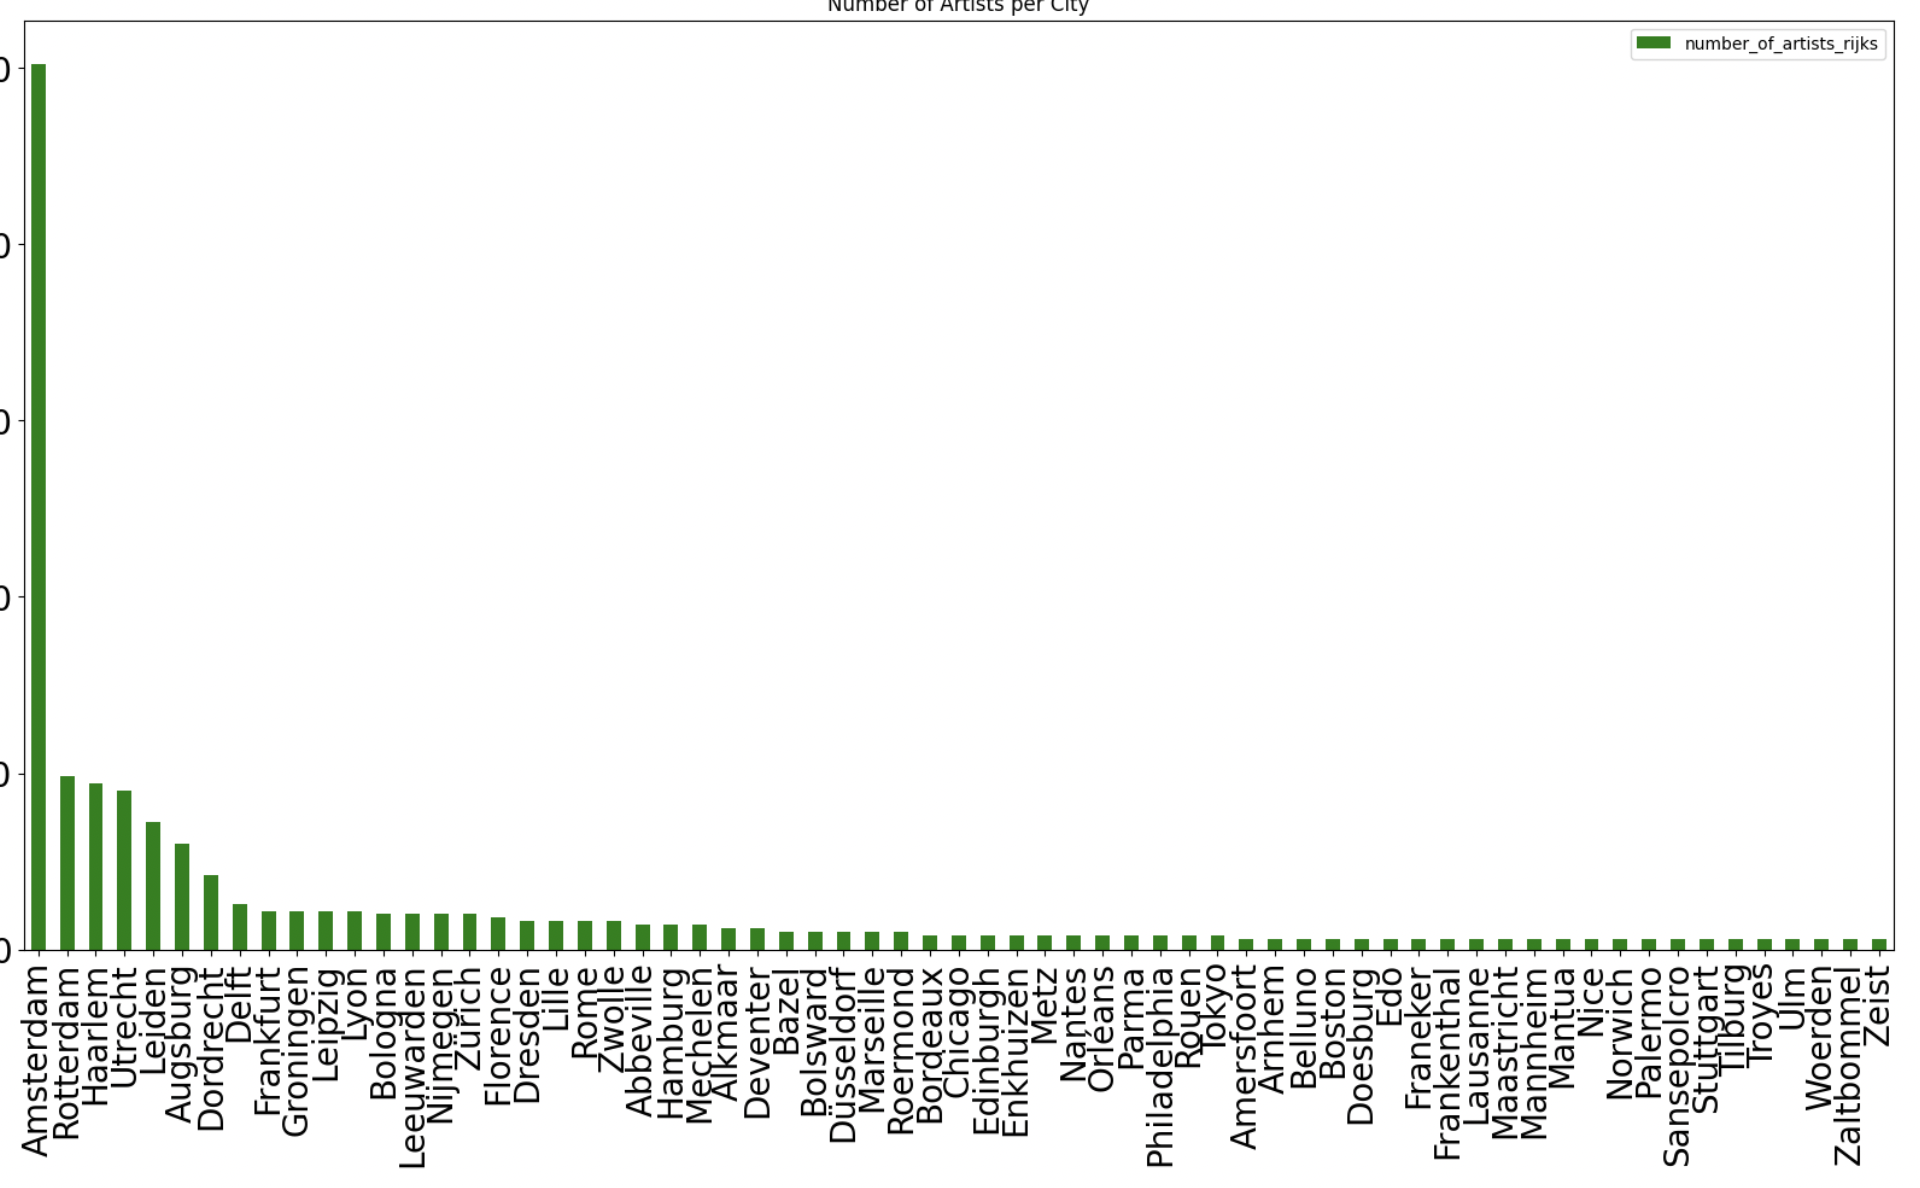
\includegraphics[scale=0.4]{bonus.png}
\newline
\caption{Figure 9: Bar graph visualisation of first query.}
\end{center}

As for the second query we decided that the best way to display this kind of data is with a help of a map - using the folium package for python. That is why we've come up with the following interactive representation of the matter. 

\begin{center}
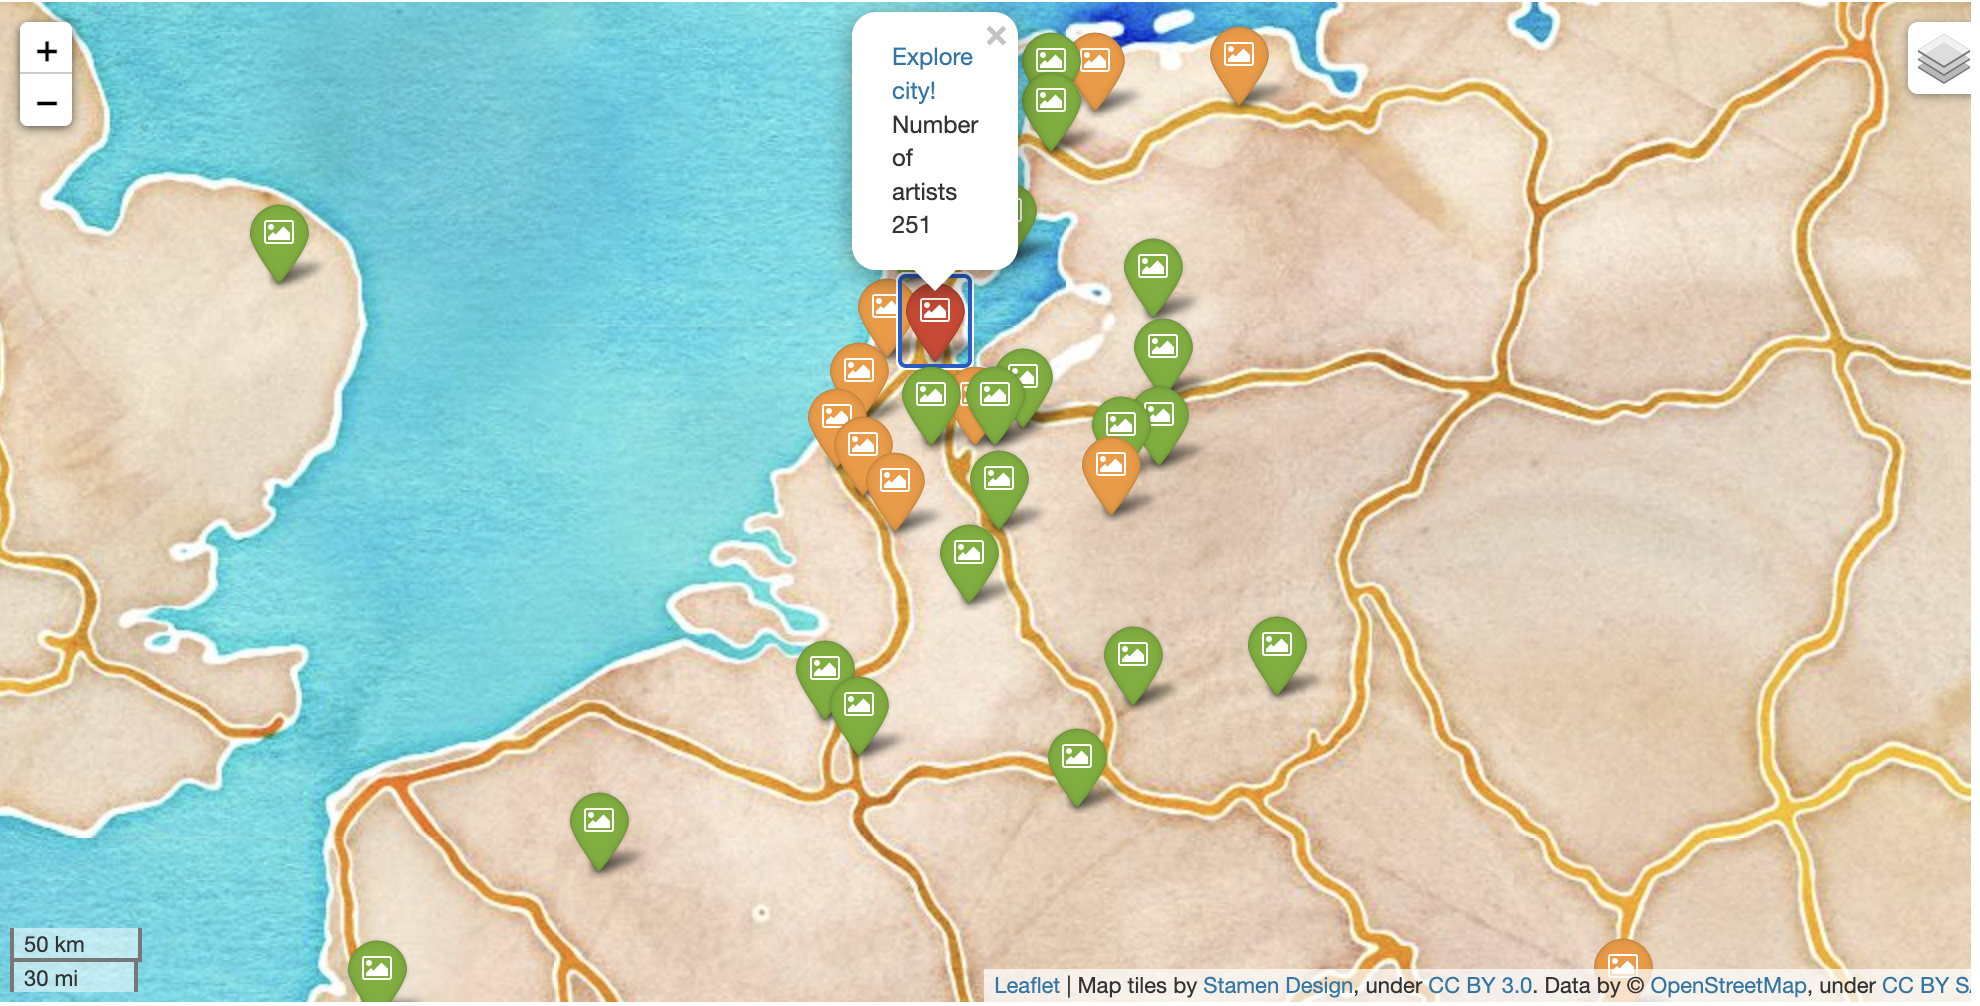
\includegraphics[scale=0.4]{map.png}
\newline
\caption{Figure 10: Example image from our map visualisation of the second query.}
\end{center}
\bibliography{refs}
\bibliographystyle{ieeetr}

\end{document}

